% ****** Start of file apssamp.tex ******
%
%   This file is part of the APS files in the REVTeX 4.1 distribution.
%   Version 4.1r of REVTeX, August 2010
%
%   Copyright (c) 2009, 2010 The American Physical Society.
%
%   See the REVTeX 4 README file for restrictions and more information.
%
% TeX'ing this file requires that you have AMS-LaTeX 2.0 installed
% as well as the rest of the prerequisites for REVTeX 4.1
%
% See the REVTeX 4 README file
% It also requires running BibTeX. The commands are as follows:
%
%  1)  latex apssamp.tex
%  2)  bibtex apssamp
%  3)  latex apssamp.tex
%  4)  latex apssamp.tex
%
\documentclass[%
 reprint,
%superscriptaddress,
%groupedaddress,
%unsortedaddress,
%runinaddress,
%frontmatterverbose, 
%preprint,
%showpacs,preprintnumbers,
%nofootinbib,
%nobibnotes,
%bibnotes,
 amsmath,amssymb,
 aps,
%pra,
%prb,
%rmp,
%prstab,
%prstper,
%floatfix,
spanish]{revtex4-1}

\usepackage{graphicx}% Include figure files
\usepackage{dcolumn}% Align table columns on decimal point
\usepackage{bm}% bold math
\usepackage{subcaption}
\usepackage[utf8]{inputenc}
%\usepackage{hyperref}% add hypertext capabilities
%\usepackage[mathlines]{lineno}% Enable numbering of text and display math
%\linenumbers\relax % Commence numbering lines

%\usepackage[showframe,%Uncomment any one of the following lines to test 
%%scale=0.7, marginratio={1:1, 2:3}, ignoreall,% default settings
%%text={7in,10in},centering,
%%margin=1.5in,
%%total={6.5in,8.75in}, top=1.2in, left=0.9in, includefoot,
%%height=10in,a5paper,hmargin={3cm,0.8in},
%]{geometry}
\graphicspath{ {imagenes/} }
\begin{document}

\preprint{APS/123-QED}

\title{Percolaci\'on de nodos en redes cuadradas 2d}% Force line breaks with \\
%\thanks{A footnote to the article title}%

\author{A.~Rabinovich}
 %\altaffiliation[Also at ]{}%Lines break automatically or can be forced with \\
\affiliation{%
 Departamento de F\'\i sica, Facultad de Ciencias Exactas y Naturales, Universidad de Buenos Aires,\\
 Pabell\'on I, Ciudad Universitaria, 1428 Buenos Aires, Argentina.
}%

%\collaboration{MUSO Collaboration}%\noaffiliation

\date{\today}% It is always \today, today,
             %  but any date may be explicitly specified

\begin{abstract}
A partir de estudios computacionales hemos determinado el comportamiento cr\'\i tico de una red de nodos bi-dimensional. Esta red percola siguiendo una transici\'on de fase de $2^\circ$ orden .... 


\begin{description}
%\item[Usage]
%Secondary publications and information retrieval purposes.
\item[PACS numbers]
45.70.Vn, 89.65.Lm
%\item[Structure]
%You may use the \texttt{description} environment to structure your abstract;
%use the optional argument of the \verb+\item+ command to give the category of each item. 
\end{description}
\end{abstract}

\pacs{45.70.Vn, 89.65.Lm}% PACS, the Physics and Astronomy
                             % Classification Scheme.
%\keywords{Suggested keywords}%Use showkeys class option if keyword
                              %display desired
\maketitle

%\tableofcontents

\section{\label{intro}Introducci\'on}

Los primeros estudios en percolaci\'on se realizaron....


\section{\label{theory}El modelo}



\subsection{\label{transition}Transici\'on de fase}

Cuando de var\'\i a la probabilidad de ocupaci\'on de los nodos de la red, se observa que ...

\subsection{\label{critical}Leyes de potencia y exponentes cr\'\i ticos}

La Tabla~\ref{table_1} resume las principales leyes de potencia obtenidas en la literatura para redes percolantes...

\begin{table}[h]
\caption{\label{table_1}%
Valores te\'oricos hallados en la literatura.
}
\begin{ruledtabular}
\begin{tabular}{lll}
%\hline
%\hline
\\[-5pt]
 S\'\i mbolo     & Ley                        & Valor                          \\
\hline
$d$             &   ---                         & $d=2$                        \\
$D$             & $M\sim L^{D}$                 & $D=91/48$                    \\
$\nu$           & $\xi\sim|p-p_c|^{-\nu}$       & $\nu=4/3$                    \\
$\tau$          & $n(p_c)\sim s^{-\tau}$        & $\tau=1+d/D$                 \\
$\sigma$        & $z=s^\sigma(p-p_c)$           & $\sigma=(\nu D)^{-1}$        \\
$\alpha$        & $m_0(p)\sim|p-p_c|^{2-\alpha}$& $\alpha=2-(\tau-1)/\sigma$   \\
$\beta$         & $m_1(p)\sim(p-p_c)^\beta$     & $\beta=\nu(d-D)$             \\
$\gamma$        & $m_2(p)\sim|p-p_c|^{-\gamma}$ & $\gamma=(3-\tau)/\sigma$     \\
%\hline
\end{tabular}
\end{ruledtabular}
\end{table}

Observamos que los valores obtenidos en la Ref.~\cite{Stauffer} presentan...



\subsection{\label{scaling}Efectos de red finita}

El comportamiento de las redes de tama\~no finito (redes cuadradas de lado $L$) se aparta de aquel esperado para sistemas infinitos. Esto se debe a que...


\begin{equation}
n_s(p)=q_0\,s^{-\tau}\,f(z)\ \ \ \ ,\ \ \ \ z=s^\sigma(p-p_c)\label{eqn_1}
\end{equation}

En la Ec.~(\ref{eqn_1}) ....

\subsection{\label{renorm}Renormalizaci\'on}

Es posible explotar a\'un m\'as el hecho de que cerca de la transici\'on de fase el sistema se muestra libre de escalas. Si se \emph{re-escala} el sistema, deben seguir siendo v\'alidas las leyes de potencia anteriores. Entonces, mediante un proceso de \emph{renormalizaci\'on} observaremos que...

\section{\label{simulations}Simulaciones num\'ericas}

Se estudiaron redes cuadradas de tama\~no $L=4, 16, 32, 64, 128$ por medio del algoritmo de Hoshen-Kopelman \cite{Kopelman}. 


\begin{equation}
M(L)=L^D\,m\bigg(\displaystyle\frac{L}{\xi}\bigg)\sim\left\{\begin{array}{lll}
             L^D       & \textrm{si} & L<\xi \\
             L^d       & \textrm{si} & L\gg\xi \\
            \end{array}\right.\label{eqn_2}
\end{equation}


\section{\label{results}Resultados}

\subsection{\label{p_c} Determinaci\'on de $p_c$ por diferentes m\'etodos}

Se usaron distintos m\'etodos para la determinaci\'on num\'erica del punto cr\'\i tico...(\emph{i.e.} b\'usqueda de $p_\mathrm{medio}$, b\'usqueda de $p_\mathrm{mediana}$, sintonizado de $n_s(p_c)$).

a)

\begin{figure}[h]
\begin{subfigure}{.25\textwidth}
  \centering
  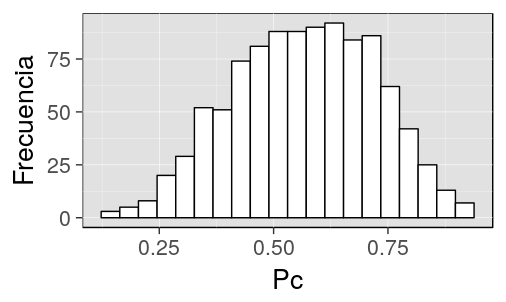
\includegraphics[width=.9\linewidth]{ej1a/hist4x4}
  \caption{Red cuadrada de 4x4: $\mu=0.5669$ $\sigma=0.1554$}
  %\caption{Red cuadrada de 4x4: $P_c=0.5\pm0.2$}
  \label{fig:1a4x4}
\end{subfigure}%
\begin{subfigure}{.25\textwidth}
  \centering
  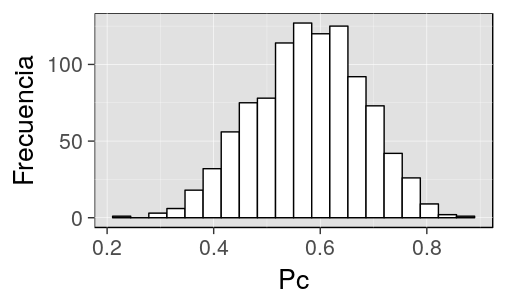
\includegraphics[width=.9\linewidth]{ej1a/hist8x8}
  \caption{Red cuadrada de 8x8: $\mu=0.5779$ $\sigma=0.1018$}
  %\caption{Red cuadrada de 8x8: $P_c=0.5\pm0.1$}
  \label{fig:1a8x8}
\end{subfigure}
\begin{subfigure}{.25\textwidth}
  \centering
  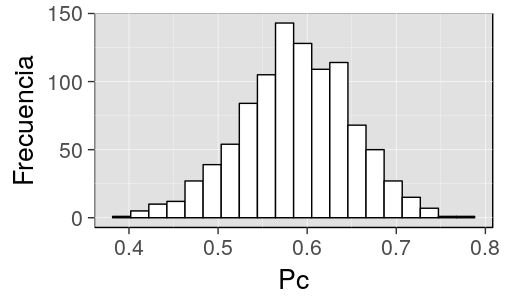
\includegraphics[width=.9\linewidth]{ej1a/hist16x16}
  \caption{Red cuadrada de 16x16: $\mu=0.5876$ $\sigma=0.0620$}
  %\caption{Red cuadrada de 16x16: $P_c=0.58\pm0.06$}  
  \label{fig:1a16x16}
\end{subfigure}%
\begin{subfigure}{.25\textwidth}
  \centering
  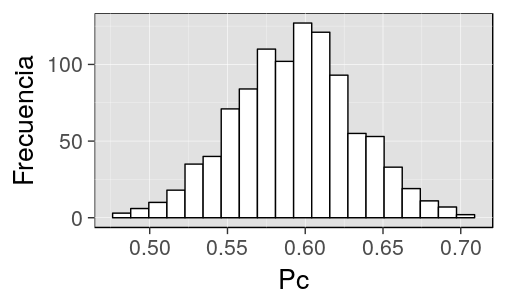
\includegraphics[width=.9\linewidth]{ej1a/hist32x32}
  \caption{Red cuadrada de 32x32: $\mu=0.5932$ $\sigma=0.0390$}
  %\caption{Red cuadrada de 32x32: $P_c=0.59\pm0.04$}  
  \label{fig:1a32x32}
\end{subfigure}
\begin{subfigure}{.25\textwidth}
  \centering
  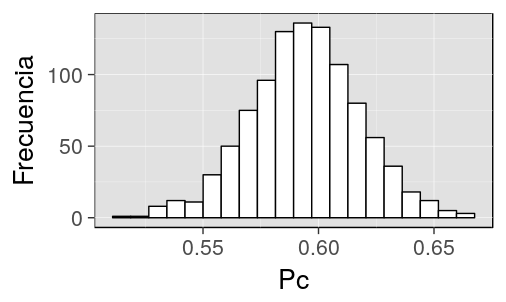
\includegraphics[width=.9\linewidth]{ej1a/hist64x64}
  \caption{Red cuadrada de 64x64: $\mu=0.5940$ $\sigma=0.0239$}
  %\caption{Red cuadrada de 64x64: $P_c=0.59\pm0.02$}  
  \label{fig:1a64x64}
\end{subfigure}%
\begin{subfigure}{.25\textwidth}
  \centering
  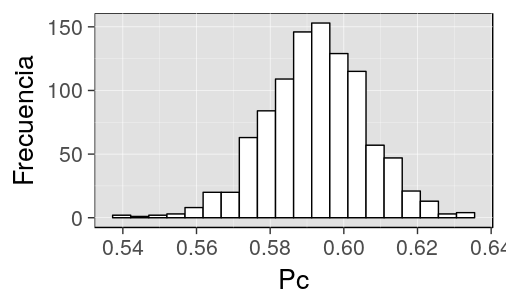
\includegraphics[width=.9\linewidth]{ej1a/hist128x128}
  \caption{Red cuadrada de 128x128: $\mu=0.5924$ $\sigma=0.0137$}
  %\caption{Red cuadrada de 128x128: $P_c=0.59\pm0.01$}  
  \label{fig:1a128x128}
\end{subfigure}
\caption{Histogramas de probabilidades críticas en función del tamaño de la red cuadrada para 1000 realizaciones de la red.}
\label{fig:histograma_red_cuadrada_1a}
\end{figure}

b)

\begin{figure}[h]
\begin{subfigure}{.25\textwidth}
  \centering
  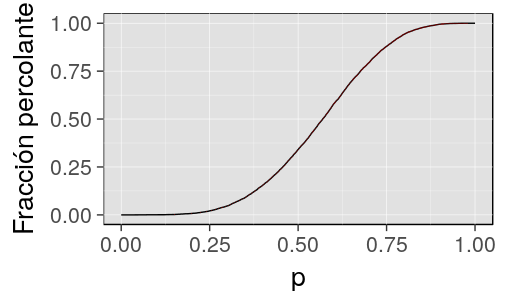
\includegraphics[width=.9\linewidth]{ej1b/4x4}
  %\caption{Red cuadrada de 4x4: $\mu=0.569$ $\sigma=0.006$}
  \caption{Red cuadrada de 4x4: $P_c=0.569\pm0.003$}
  \label{fig:1b4x4}
\end{subfigure}%
\begin{subfigure}{.25\textwidth}
  \centering
  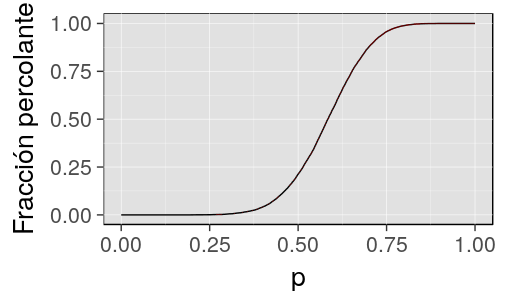
\includegraphics[width=.9\linewidth]{ej1b/8x8}
  %\caption{Red cuadrada de 8x8: $\mu=0.584$ $\sigma=0.002$}
  \caption{Red cuadrada de 8x8: $P_c=0.584\pm0.003$}
  \label{fig:1b8x8}
\end{subfigure}
\begin{subfigure}{.25\textwidth}
  \centering
  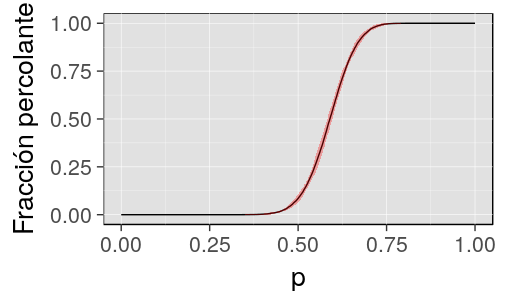
\includegraphics[width=.9\linewidth]{ej1b/16x16}
  %\caption{Red cuadrada de 16x16: $\mu=0.589$ $\sigma=0.003$}
  \caption{Red cuadrada de 16x16: $P_c=0.590\pm0.003$}  
  \label{fig:1b16x16}
\end{subfigure}%
\begin{subfigure}{.25\textwidth}
  \centering
  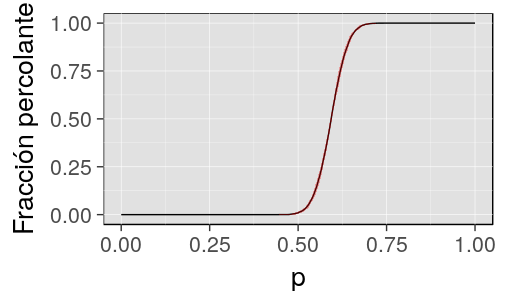
\includegraphics[width=.9\linewidth]{ej1b/32x32}
  %\caption{Red cuadrada de 32x32: $\mu=0.593$ $\sigma=0.001$}
  \caption{Red cuadrada de 32x32: $P_c=0.593\pm0.003$}  
  \label{fig:1b32x32}
\end{subfigure}
\begin{subfigure}{.25\textwidth}
  \centering
  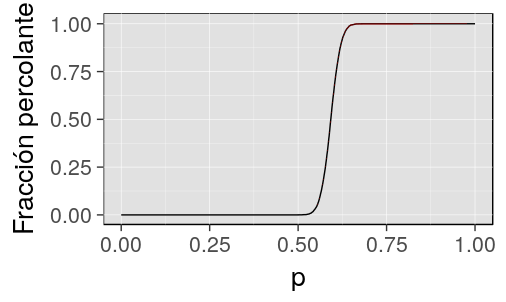
\includegraphics[width=.9\linewidth]{ej1b/64x64}
  %\caption{Red cuadrada de 64x64: $\mu=0.5927$ $\sigma=0.0006$}
  \caption{Red cuadrada de 64x64: $P_c=0.592\pm0.003$}  
  \label{fig:1b64x64}
\end{subfigure}%
\begin{subfigure}{.25\textwidth}
  \centering
  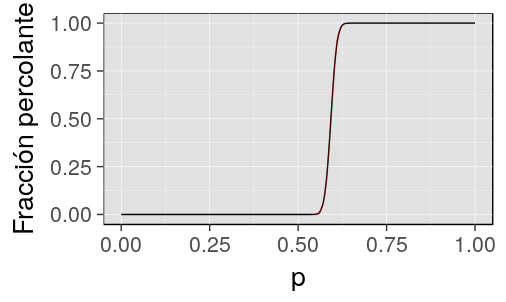
\includegraphics[width=.9\linewidth]{ej1b/128x128}
  %\caption{Red cuadrada de 128x128: $\mu=0.5931$ $\sigma=0.0005$}
  \caption{Red cuadrada de 128x128: $P_c=0.593\pm0.003$}  
  \label{fig:1b128x128}
\end{subfigure}
\caption{Histogramas de probabilidades críticas en función del tamaño de la red cuadrada para 1000 realizaciones de la red.}
\label{fig:1b}
\end{figure}

d)

Red cuadrada de 16x16: $P_c=0.594\pm0.001$
Red cuadrada de 32x32: $P_c=0.595\pm0.003$
Red cuadrada de 64x64: $P_c=0.594\pm0.003$
Red cuadrada de 128x128: $P_c=0.594\pm0.003$

\subsection{\label{2} Intensidad del cluster percolante $P_c$}

\begin{figure}[h]
\begin{subfigure}{.25\textwidth}
  \centering
  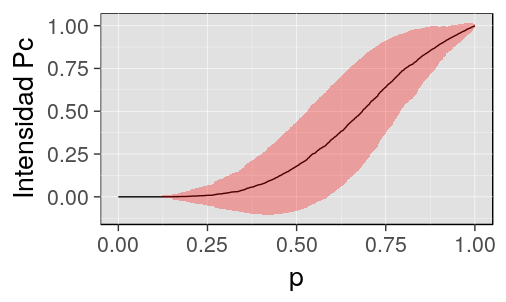
\includegraphics[width=.9\linewidth]{ej2/4x4}
  %\caption{Red cuadrada de 4x4: $\mu=0.569$ $\sigma=0.006$}
  %\caption{Red cuadrada de 4x4: $P_c=0.569\pm0.003$}
  \label{fig:24x4}
\end{subfigure}%
\begin{subfigure}{.25\textwidth}
  \centering
  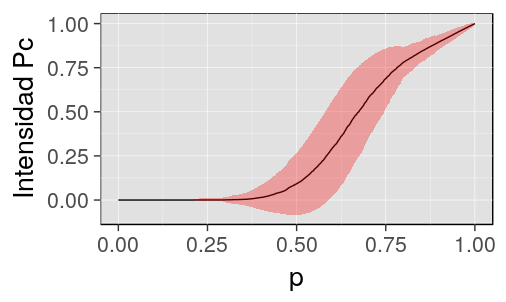
\includegraphics[width=.9\linewidth]{ej2/8x8}
  %\caption{Red cuadrada de 8x8: $\mu=0.584$ $\sigma=0.002$}
  %\caption{Red cuadrada de 8x8: $P_c=0.584\pm0.003$}
  \label{fig:28x8}
\end{subfigure}
\begin{subfigure}{.25\textwidth}
  \centering
  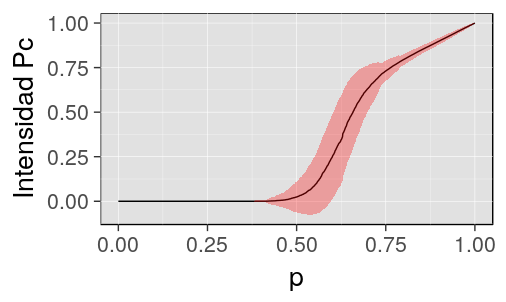
\includegraphics[width=.9\linewidth]{ej2/16x16}
  %\caption{Red cuadrada de 16x16: $\mu=0.589$ $\sigma=0.003$}
  %\caption{Red cuadrada de 16x16: $P_c=0.590\pm0.003$}  
  \label{fig:216x16}
\end{subfigure}%
\begin{subfigure}{.25\textwidth}
  \centering
  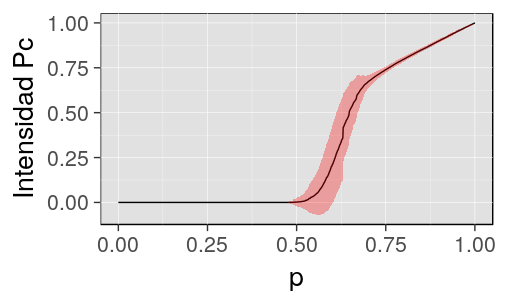
\includegraphics[width=.9\linewidth]{ej2/32x32}
  %\caption{Red cuadrada de 32x32: $\mu=0.593$ $\sigma=0.001$}
  %\caption{Red cuadrada de 32x32: $P_c=0.593\pm0.003$}  
  \label{fig:232x32}
\end{subfigure}
\begin{subfigure}{.25\textwidth}
  \centering
  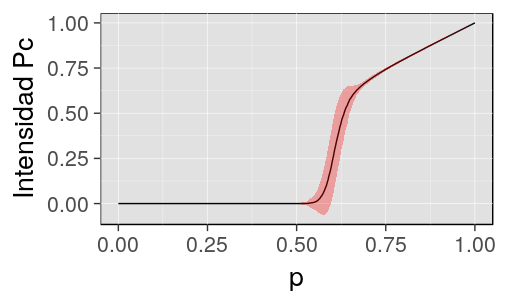
\includegraphics[width=.9\linewidth]{ej2/64x64}
  %\caption{Red cuadrada de 64x64: $\mu=0.5927$ $\sigma=0.0006$}
  %\caption{Red cuadrada de 64x64: $P_c=0.592\pm0.003$}  
  \label{fig:264x64}
\end{subfigure}%
\begin{subfigure}{.25\textwidth}
  \centering
  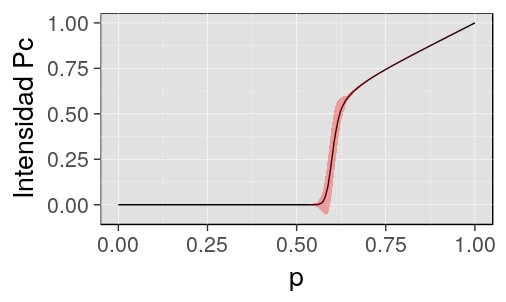
\includegraphics[width=.9\linewidth]{ej2/128x128}
  %\caption{Red cuadrada de 128x128: $\mu=0.5931$ $\sigma=0.0005$}
  %\caption{Red cuadrada de 128x128: $P_c=0.593\pm0.003$}  
  \label{fig:2128x128}
\end{subfigure}
\caption{Intensidad del cluster percolante en función de p y del tamaño de la red cuadrada para 1000 realizaciones de la red.}
\label{fig:2}
\end{figure}

\subsection{\label{3} Determinaci\'on de la dimensi\'on fractal $D$ }

\begin{figure}[h]
  \centering
  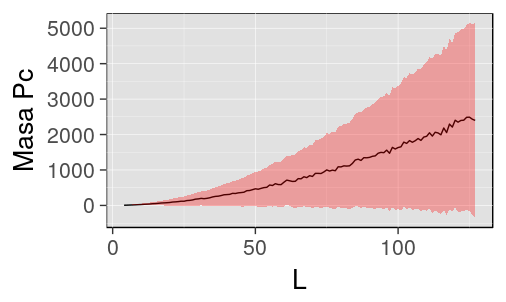
\includegraphics[width=.9\linewidth]{ej3/masa}
  \label{fig:2masa}
\caption{Masa del cluster percolante $P_c$ en función del tamaño de la red cuadrada para 1000 realizaciones de la red.}
\label{fig:3}
\end{figure}


\subsection{\label{D} Determinaci\'on de la dimensi\'on fractal $D$ }

Seg\'un la Ec.~\ref{eqn_2} es posible hallar $D$ en el caso en que ....

\subsection{\label{P} Obtenci\'on de $\beta$ a partir de la intensidad $P_\infty$}

A partir de la informaci\'on en el gr\'afico de $P_\infty(p)$ podemos hallar $\beta$ ...

\subsection{\label{S} Espectro de fragmentos y verficaci\'on de la hip\'otesis de \emph{scaling} }

La hip\'otesis de \emph{scaling} se presenta en la Ec.~\ref{eqn_1} en donde se observa que para distintos valores de $s$ y $p-p_c$, el espectro de fragmentos debe colapsar en una \'unica curva $f(z)=n_s(p)/n_s(p_c)$, donde $z=s^\sigma(p-p_c)$.... 

\begin{figure}[b]
\begin{center}
%\includegraphics[scale=0.62]{fig1} \\
\caption{Distribuci\'on de fragmentos.... }\label{fig_1}
\end{center}
\end{figure}

En la Fig.~\ref{fig_1} se observa que ... \\


En consecuencia, verificamos la hip\'otesis de \emph{scaling} graficando $f(z)$  y determinando el punto $f_\mathrm{max}=f(z_\mathrm{max})$. Este valor se corresponde con una probabilidad $p_\mathrm{max}$ para un cada tama\~no $s$ fijo. La ley de potencia con exponente $\sigma$ ser\'a entonces

 
\begin{equation}
\ln(p_\mathrm{max}-p_c)=-\sigma\,\ln(s)+\ln(z_\mathrm{max})+C\label{eqn_3}
\end{equation}


\section{\label{R} Verificaci\'on de resultados por renormalizaci\'on}

Podemos verificar, al menos de manera aproximada, los resulados del las secciones realizando un proceso de renormalzaci\'on de \emph{celda peque\~na}. Consideramos un porci\'on de red de lado $b=2$ y la llamamos un \emph{super-nodo}....

\section{\label{conclusions}Conclusiones}

La Tabla.... resume los resulatados obtenidos. El sistema ....


\begin{acknowledgments}
A. Rabinovich es becario doctoral del CONICET. 
\end{acknowledgments}

\appendix
%\bibliography{apssamp}% Produces the bibliography via BibTeX.
\bibliography{apspaper}% Produces the bibliography via BibTeX.

\end{document}
%
% ****** End of file apssamp.tex ******
